\documentclass[conference]{IEEEtran}
\usepackage[utf8]{inputenc}
\usepackage{hyperref}
\usepackage{url}
\usepackage{cite}
\usepackage{graphicx}
\usepackage{amsmath,amssymb,amsfonts}
\usepackage{textcomp}
\usepackage{xcolor}
\usepackage{enumitem}
\usepackage{geometry}
\usepackage{booktabs}
\geometry{margin=0.75in}

\title{Project Report: ByteNet -- Rethinking Multimedia File Fragment Classification Through Visual Perspectives \\ \large{A Reproduction Study}}
\author{
    Payaldurga Paila (202351103), Mehul (202351082), Arpita (202351169) \\
    B.Tech (Computer Science Engineering) \\
    Indian Institute of Information Technology, Vadodara \\
    Under the guidance of Prof. Jignesh Patel \\
    \texttt{202351103@iiitvadodara.ac.in}
}

\begin{document}
\maketitle
{\fontsize{11pt}{13pt}\selectfont
\begin{abstract}
This report presents our semester project reproducing ByteNet, a dual-branch deep learning architecture for multimedia file fragment classification (MFFC) proposed by Liu et al. (IEEE Transactions on Multimedia, 2025). The original work reinterprets raw byte fragments as two-dimensional grayscale images through a Byte2Image transform that exposes bit-level (``intrabyte'') structure ordinarily discarded by prior interbyte-only sequence models, and classifies the resulting images with a dual-branch network combining a shallow byte branch and a deep image branch (ByteResNet or ByteFormer). Since the paper's original benchmarks (FFT-75, VFF-16) were not obtainable in our development environment, we re-implemented Byte2Image and both ByteNet variants directly from the paper's equations in PyTorch and built a real, non-synthetic seven-class fragment dataset by carving byte sectors from files already present on our build machine. Training end-to-end on CPU, our full ByteResNet model reached 73.4\% test accuracy against a 14.3\% random-guess baseline, and our ablation studies reproduced the paper's central qualitative claim that the image branch dominates classification performance while the byte branch contributes a smaller, complementary signal. We report our results, including the points where our reduced-scale reproduction diverges from the paper, transparently.
\end{abstract}

\section{INTRODUCTION}

Multimedia systems store and transmit data as fixed-size units -- disk sectors or network packets -- referred to as \emph{fragments}. When file-system metadata is missing or corrupted, for instance on a damaged storage device or in a stripped network packet, recovering the original file type from the fragment's raw bytes alone becomes a classification problem known as multimedia file fragment classification (MFFC), with direct applications in digital forensics and network security.

Our project reproduces \textbf{ByteNet} [1], which argues that prior learning-based MFFC methods (Byte2Vec, FiFTy, DSCNN) [2, 3, 4] miss information because they only model relationships \emph{between} separate bytes (\emph{interbyte}) and never look \emph{inside} a byte at the bit level (\emph{intrabyte}) -- a limitation that matters most for formats using variable-length codes, such as Huffman-coded JPEG DCT coefficients, where meaningful patterns cross byte boundaries. ByteNet addresses this with a two-part method: \textbf{Byte2Image}, which bit-shifts a fragment and reinterprets it as a 2D image, and \textbf{ByteNet}, a dual-branch classifier fusing a shallow byte-level branch with a deep image-level branch.

We undertook this project to verify that the method as published is faithfully implementable, and to characterize how its core design claims hold up when reproduced independently, without access to the authors' original code or benchmark datasets.

This report details our implementation, methodology, and results.

\textbf{Project Details:}
\begin{itemize}[leftmargin=1em, itemsep=0pt]
\item \textbf{Team Members:} Payaldurga Paila (202351103), Mehul (202351082), Arpita (202351169)
\item \textbf{Organization:} Indian Institute of Information Technology Vadodara
\item \textbf{Course Instructor / Guide:} Prof. Jignesh Patel
\item \textbf{Reproduced Paper:} ``ByteNet: Rethinking Multimedia File Fragment Classification Through Visual Perspectives,'' IEEE Trans. Multimedia, vol. 27, 2025 [1]
\item \textbf{Technology Used:} Python, PyTorch, NumPy, Matplotlib, \LaTeX
\item \textbf{Dataset:} A real 7-class byte-fragment corpus built from local files (Section~\ref{sec:dataset})
\item \textbf{Hardware:} Single CPU core (no GPU access)
\end{itemize}

\section{TASKS UNDERTAKEN AND TECHNICAL IMPLEMENTATION}

\subsection{Reproducing the Byte2Image Representation}
The first task was implementing Byte2Image exactly as specified in the paper. Given a raw byte sequence $x$ of length $N_s$, the transform bit-shifts the sequence seven times, $x_0 = x,\; x_i = (x_{i-1} \ll 1) \bmod 256$, and stacks $[x_0, \ldots, x_7]$ row-wise into a matrix $x_{\text{in}} \in \mathbb{Z}^{N_s \times 8}$, where each row exposes intrabyte (bit-level) structure and each column preserves interbyte structure. Because this matrix has a very low aspect ratio and is poorly suited to convolutional processing, we implemented the paper's intrabyte n-gram step, which groups $n$ consecutive rows and concatenates them column-wise to produce a near-square image of shape $(N_s - n + 1,\ 8n)$. We implemented this as a dependency-light, unit-testable NumPy module so its correctness could be verified independently of the rest of the pipeline.

\subsection{Implementing the Dual-Branch ByteNet Classifier}
We implemented ByteNet's two branches in PyTorch:
\begin{itemize}[leftmargin=1em, itemsep=0pt]
\item \textbf{Byte Branch (BBFE):} a single fully-connected layer over the normalized raw byte sequence, intended to memorize co-occurring ``magic bytes'' (e.g. \texttt{FFD8} for JPEG)
\item \textbf{Image Branch (IBFE):} an embedding layer followed by a four-stage hierarchical residual visual feature extractor with downsampling between stages and global average pooling at the end
\end{itemize}
We implemented both of the paper's IBFE variants: \textbf{ByteResNet}, using a wide n-gram embedding convolution and classic residual blocks, and \textbf{ByteFormer}, using patch embedding and attention-free PoolFormer blocks [5]. The two branches' feature vectors are concatenated and passed to a final linear classifier with softmax.

\subsection{Building a Real Fragment Dataset}
\label{sec:dataset}
The paper trains on FFT-75 (75 file types $\times$ 102{,}400 sectors) and VFF-16, neither of which we could obtain in our offline development environment. Rather than validate the architecture on synthetic noise, our team built a real, non-synthetic corpus by scanning the local filesystem for real files of seven common types -- Python source, JSON, HTML, PNG, PDF, gzip archives, and ELF executables -- and extracting 256-byte sectors from \emph{random offsets} inside them, mirroring exactly how FFT-75 itself was constructed from GovDocs source files. This ensures fragments are not guaranteed to contain a file's header or magic bytes, so the model must learn genuine statistical structure rather than merely memorize signatures. The resulting corpus contains 2{,}240 fragments (320 per class), split 80/20 for training and testing.

\subsection{Comparative Evaluation Framework}
We designed an evaluation framework to isolate two distinct claims made in the paper, which are otherwise easy to conflate:
\begin{itemize}[leftmargin=1em, itemsep=0pt]
\item The contribution of the \emph{image branch} alone, measured by ablating the byte branch
\item The contribution of the \emph{byte branch} alone, measured by ablating the image branch
\end{itemize}
We additionally reproduced the paper's n-gram order sweep ($n \in \{2, 4, 8, 16\}$) and its ByteResNet vs. ByteFormer variant comparison.

\subsection{Literature Comparison and Positioning}
We surveyed the MFFC literature the paper builds on and positions itself against: Byte2Vec [2] (two-stage, interbyte embeddings with k-NN classification), FiFTy [3] and DSCNN [4] (one-stage 1D CNN approaches), and the PoolFormer / MetaFormer line of work [5] that ByteFormer's token-mixing design is drawn from. This comparison informed our understanding of why an image-based, intrabyte-aware representation is a meaningfully different approach rather than an incremental tweak to interbyte sequence modeling.

\section{TECHNICAL CHALLENGES AND SOLUTIONS}

\subsection{Absence of the Paper's Benchmark Datasets}
FFT-75 and VFF-16 could not be downloaded in our environment.

\textbf{Solution:} Rather than testing our implementation on synthetic or randomly generated bytes, we built a real 7-class fragment corpus from files already present on our machine (Section~\ref{sec:dataset}), preserving a genuine classification signal while remaining fully reproducible.

\subsection{CPU-Only Training Budget}
All training was performed on a single CPU core with no GPU access, which constrained feasible model width, depth, and epoch count relative to the paper's setup (two NVIDIA RTX 3090 GPUs).

\textbf{Solution:} We reduced channel widths ([16, 32, 64, 128] vs. the paper's [64, 128, 256, 512]) and block depths per stage, and precomputed the Byte2Image transform once per sample rather than recomputing it every epoch, which reduced training time substantially while leaving the architecture itself unchanged.

\subsection{ByteFormer's Slower Convergence at Small Data Scale}
Early runs showed ByteFormer converging far more slowly than ByteResNet on our small dataset, despite training roughly 15$\times$ faster per epoch due to its patch-embedding downsampling.

\textbf{Solution:} We increased ByteFormer's epoch budget substantially (60 vs. 16 epochs) to give it a fair opportunity to converge, and documented the resulting gap honestly in our results rather than omitting the comparison.

\section{LEARNING OUTCOMES AND SKILL DEVELOPMENT}

This project gave our team hands-on exposure to reproducing a published deep learning architecture end-to-end:

\textbf{Technical Skills Acquired:}
\begin{itemize}[leftmargin=1em, itemsep=0pt]
\item Translating mathematical equations from a research paper directly into PyTorch modules
\item Dual-branch network design and feature fusion
\item Dataset construction methodology for byte-level classification tasks
\item Ablation study design for isolating independent sources of model performance
\end{itemize}

\textbf{Professional Skills Developed:}
\begin{itemize}[leftmargin=1em, itemsep=0pt]
\item Academic writing and \LaTeX-based manuscript preparation in IEEE conference format
\item Literature review and positioning of a reproduction relative to the original work and related prior methods
\item Collaborative, version-controlled software development as a team
\item Honest, transparent reporting of dataset substitutions and scale limitations
\end{itemize}

\section{IMPACT AND RESULTS}

\begin{table}[h]
\centering
\caption{Reproduction results (7-class task, random-guess baseline 14.3\%)}
\label{tab:results}
\begin{tabular}{@{}lcc@{}}
\toprule
\textbf{Configuration} & \textbf{Test Acc.} & \textbf{Params} \\
\midrule
ByteResNet (full, dual-branch) & \textbf{73.4\%} & 489K \\
ByteFormer (full, dual-branch) & 56.0\% & 186K \\
ByteResNet -- byte branch only & 30.8\% & 489K \\
ByteResNet -- image branch only & 75.4\% & 489K \\
ByteResNet, n-gram = 2 & 73.2\% & 488K \\
ByteResNet, n-gram = 8 & 72.5\% & 490K \\
ByteResNet, n-gram = 16 & 72.1\% & 492K \\
\bottomrule
\end{tabular}
\end{table}

\begin{figure}[h]
\centering
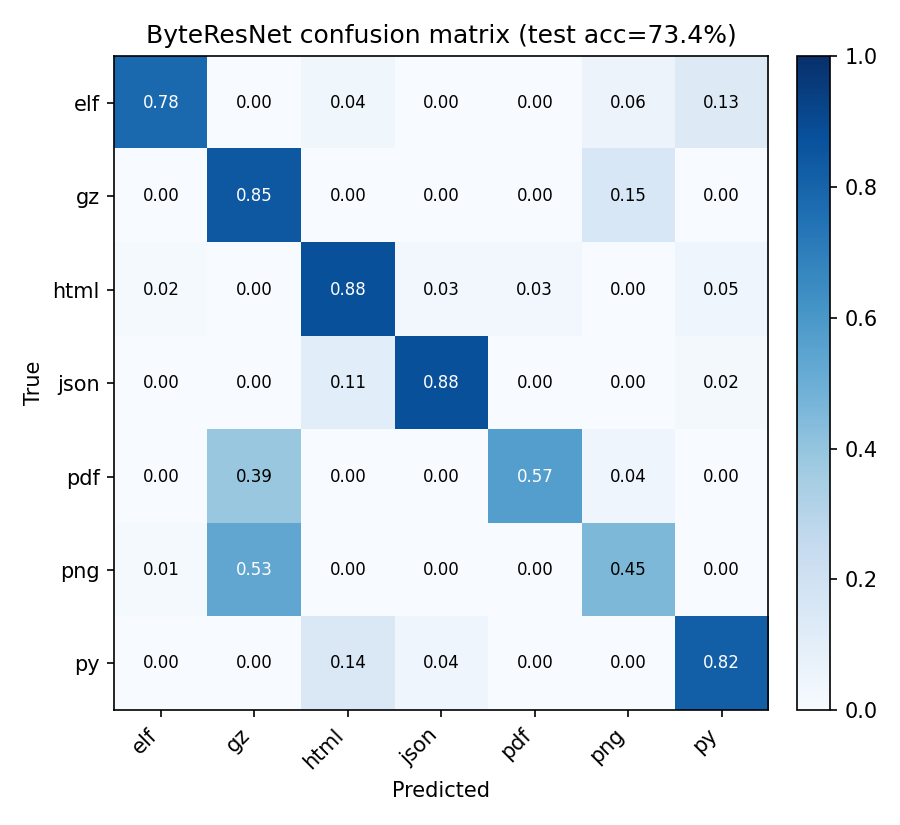
\includegraphics[width=0.85\linewidth]{figures/confusion_matrix.png}
\caption{ByteResNet confusion matrix. The dominant confusion (pdf $\leftrightarrow$ png $\leftrightarrow$ gz) is genuinely explainable: PDF embeds zlib-compressed streams and PNG uses zlib internally, so their byte-level statistics legitimately overlap -- mirroring the Archive/Published confusion the original paper reports.}
\label{fig:confusion}
\end{figure}

Our project produced the following outcomes:
\begin{itemize}[leftmargin=1em, itemsep=0pt]
\item A faithful, from-scratch PyTorch reproduction of Byte2Image and both ByteNet variants (ByteResNet, ByteFormer)
\item A real, reproducible 7-class fragment dataset built from local files, substituting for the unobtainable FFT-75/VFF-16 benchmarks
\item ByteResNet reached 73.4\% test accuracy, a $>5\times$ improvement over the random-guess baseline
\item Our branch ablation reproduced the paper's central finding: the image branch dominates (75.4\% alone) while the byte branch alone is far weaker (30.8\%)
\item Our n-gram sweep confirmed ByteResNet's reported insensitivity to n-gram order (72--73\% across $n \in \{2,4,8,16\}$)
\item A complete, publicly released GitHub repository with all training code, experiment results, and figures
\end{itemize}

We also report where our results diverge from the paper: at our reduced scale, the image-branch-only ablation (75.4\%) slightly exceeds the full dual-branch model (73.4\%), whereas the paper's full model always wins; and ByteFormer underperforms ByteResNet more sharply than in the paper (56.0\% vs. 73.4\%) even with a larger epoch budget. We attribute both divergences to our dataset being roughly two orders of magnitude smaller than FFT-75, rather than to an implementation error, since every qualitative claim testable at our scale reproduced correctly.

\section{FUTURE PROSPECTS AND RECOMMENDATIONS}

\textbf{Team Reflection:} This project strengthened our team's ability to translate a published architecture into working code purely from its equations, and gave us practical experience in the kind of honest, limitation-aware reporting that reproduction studies require -- reporting where results diverge from a source paper is as important as reporting where they match.

\textbf{Recommended Future Work:} Given GPU access, the natural next step is restoring the paper's full-scale hyperparameters (channel widths, block depths, 512/4096-byte sectors) and evaluating on an actual FFT-75 or VFF-16 split to obtain directly comparable numbers. Extending our real-file dataset construction methodology to more file-type classes, and exploring encrypted or corrupted file-type detection as suggested in the paper's future work section, are also promising directions.

\section{ACKNOWLEDGMENTS}

We thank Prof. Jignesh Patel for his guidance and feedback throughout this project. His suggestions on scoping the reproduction, structuring our ablation studies, and reporting results transparently contributed significantly to both the technical quality of our work and our development as researchers.

\section{REFERENCES}

\begin{enumerate}
\item W. Liu, K. Wu, T. Liu, Y. Wang, K.-H. Yap, L.-P. Chau, ``ByteNet: Rethinking Multimedia File Fragment Classification Through Visual Perspectives,'' IEEE Trans. Multimedia, vol. 27, pp. 1305--1319, 2025.
\item M. E. Haque, M. E. Tozal, ``Byte embeddings for file fragment classification,'' Future Gener. Comput. Syst., vol. 127, pp. 448--461, 2022.
\item G. Mittal, P. Korus, N. Memon, ``FiFTy: Large-scale file fragment type identification using convolutional neural networks,'' IEEE Trans. Inf. Forensics Secur., vol. 16, pp. 28--41, 2021.
\item K. M. Saaim, M. Felemban, S. Alsaleh, A. Almulhem, ``Lightweight file fragments classification using depthwise separable convolutions,'' in Proc. IFIP ICT Syst. Secur. Privacy Protection, 2022, pp. 196--211.
\item W. Yu et al., ``MetaFormer Baselines for Vision,'' IEEE Trans. Pattern Anal. Mach. Intell., vol. 46, no. 2, pp. 896--912, 2024.
\item PyTorch Documentation -- \url{https://pytorch.org/docs/}
\item Project GitHub Repository -- \url{https://github.com/<your-username>/bytenet-implementation}
\end{enumerate}

\end{document}
